% =====================================================================
% Silent Failures in a Production LLM Agent Runtime:
% A Labelled Incident Corpus and a Detection Benchmark
%
% QA4AGENTS 2026 -- International Workshop on Quality Assurance of
% Conversational Agentic Systems, co-located with ISSRE 2026.
% IEEE Computer Society conference format (IEEEtran).
% Build: pdflatex qa4agents_workshop.tex   (run twice for cross-refs)
%
% Source of truth for prose:
%   ../submissions/qa4agents_workshop_paper.md
% Numbers frozen at study cutoff 2026-06-11 (matches arXiv:2606.14589),
% EXCEPT corpus labelling + benchmark figures, which come from the
% released artifacts.
%
% BEFORE SUBMISSION: confirm the workshop page limit on the official
% site. If the limit is 4 pages (short paper), cut in this order:
%   1. Sec. II (Related Work) to one paragraph per theme
%   2. D2-D4 in Sec. V-D to one sentence each
%   3. Sec. VI-C (incident structure) entirely
%   4. Table I to class-level summary rows
% NEVER cut: Table I concept, Sec. VII (benchmark), Sec. VIII (threats),
% the GenAI disclosure, or the 13/22 counting correction.
%
% Author: Wei Wu <wuweinanonuaa@gmail.com>, Independent Researcher.
% =====================================================================
\documentclass[conference]{IEEEtran}
\IEEEoverridecommandlockouts

\usepackage[T1]{fontenc}
\usepackage[utf8]{inputenc}
\usepackage{cite}
\usepackage{amsmath,amssymb}
\usepackage{graphicx}
\usepackage{booktabs}
\usepackage{array}
\usepackage{xcolor}
\usepackage{tikz}
\usetikzlibrary{arrows.meta,positioning,calc,fit,backgrounds}
\usepackage[hidelinks]{hyperref}

\newcommand{\failplausible}{\emph{fail-plausible}}

% Compact list spacing for the two enumerated blocks
\usepackage{enumitem}
\setlist[enumerate]{itemsep=0.15em,topsep=0.25em,parsep=0pt}
\setlist[itemize]{itemsep=0.15em,topsep=0.25em,parsep=0pt}

\begin{document}

\title{Silent Failures in a Production LLM Agent Runtime:\\
A Labelled Incident Corpus and a Detection Benchmark}

\author{\IEEEauthorblockN{Wei Wu}
\IEEEauthorblockA{\textit{Independent Researcher}\\
wuweinanonuaa@gmail.com}}

\maketitle

\begin{abstract}
Conversational agent runtimes fail in a way that classical monitoring does
not catch. When an internal error reaches a language model's context, the
model does not stop. It writes a fluent, plausible, and wrong message to the
user. We call this a \failplausible{} failure.

We report an eight-week study of one production personal-assistant runtime.
The runtime schedules about 40 jobs, routes across 8 LLM providers, and
messages a human user daily. We recorded 22 silent-failure incidents with
complete postmortems. We label each incident with a failure mechanism, a
silence span, a discovery channel, and the artifact a human could have seen.

Three measurements over this corpus: a human reading the product discovered
13 of 22 incidents (59\%); automated checks discovered 3 (14\%); silence
spans ranged from 36 minutes to 60 days. The corpus yields a five-class
mechanism taxonomy. One class, chained hallucination, has no counterpart in
the gray-failure literature.

We release the labelled corpus and a runnable benchmark for \failplausible{}
detectors. A deterministic reference detector flags 6 of 6 regression cases
with 0 false positives on 4 clean cases, and misses 4 of 4 held-out cases.
That last number is the point: pattern-based detection is a regression
engine, not a prediction engine. The benchmark exists so other teams can
measure that gap on their own systems.
\end{abstract}

\begin{IEEEkeywords}
LLM agent systems, silent failures, fault taxonomy, benchmark, runtime
monitoring
\end{IEEEkeywords}

% =====================================================================
\section{Introduction}
% =====================================================================

The reliability literature has studied failures that hide from their own
detectors. Huang et al.\ named \emph{gray failure}: a component degrades
while the health check reports success~\cite{huang2017gray}. Gunawi et al.\
documented \emph{fail-slow} hardware that throttles for hours before anyone
suspects it~\cite{gunawi2018failslow}. Both share one property. The system
suffers, and the observer built to notice does not.

LLM agent runtimes inherit this problem. They also add a new one. An agent
runtime produces language. When an upstream error leaks into its context
window, the runtime does not go quiet. It speaks.

One incident in our corpus shows the shape. A logging bug wrote HTTP error
text into a cache that a nightly synthesis job treated as input signal. The
model read error strings where topic signals were expected. It produced a
confident analysis of a ``Hugging Face platform crisis'' and pushed that
analysis to the user as a routine digest. No detector fired. Every test
passed. The error was not lost. It was narrated.

We call this failure mode \textbf{\failplausible{}}: the system converts an
internal error into output that is coherent, contextually appropriate, and
false. For an observer, \failplausible{} is worse than gray failure. Gray
failure denies the observer a signal. \failplausible{} hands the observer a
counterfeit one.

Quality assurance for conversational agentic systems has to detect this
class. Detecting it is hard for a reason that our data makes concrete: the
failures are semantic, so tests that check status codes, exit codes, and
schemas do not see them. Building detectors requires labelled examples of
real production failures, and such examples are scarce.

This paper contributes the examples and a way to measure detectors against
them.

\subsection{Research questions}

\begin{itemize}
  \item \textbf{RQ1.} What mechanisms produce silent failures in a
        production LLM agent runtime?
  \item \textbf{RQ2.} Which channel discovers these failures, and how long
        do they stay silent?
  \item \textbf{RQ3.} Can the corpus support a reproducible benchmark for
        \failplausible{} detectors, and what does a deterministic reference
        detector achieve on it?
\end{itemize}

\subsection{Contributions}

\begin{enumerate}
  \item \textbf{A labelled incident corpus} (Sec.~\ref{sec:corpus}).
        Twenty-two production silent-failure incidents, each with a full
        public postmortem and machine-readable labels: mechanism class,
        silence span, discovery channel, observable artifact, and whether
        the incident involved model fabrication.
  \item \textbf{A five-class mechanism taxonomy}
        (Sec.~\ref{sec:taxonomy}), with an explicit discriminator between
        the two classes that are easiest to confuse.
  \item \textbf{Discovery and latency measurements}
        (Sec.~\ref{sec:findings}) with explicit denominators, reported as
        descriptive counts for this system rather than as population
        estimates.
  \item \textbf{A runnable benchmark} (Sec.~\ref{sec:bench}) built from the
        corpus, with a reference detector, a published scorecard, and a
        contribution protocol for adding cases from other systems.
\end{enumerate}

All artifacts are public at
\url{https://github.com/bisdom-cell/openclaw-model-bridge}.

% =====================================================================
\section{Related Work}
% =====================================================================

\textbf{Silent failure in distributed systems.} Gray failure formalizes
differential observability: the application's experience and the detector's
view diverge~\cite{huang2017gray}. Fail-slow at scale collected 114 hardware
fault reports across institutions and documented diagnosis times in the
hundreds of hours~\cite{gunawi2018failslow}. Our study sits in this
tradition but at a different layer. The subject is an LLM agent runtime, and
every incident in the corpus is silent by construction. Two of our classes
will be familiar to that readership. One will not.

\textbf{Failure studies of LLM agents.} MAST derives 14 failure modes from
over 1{,}600 annotated traces across 7 multi-agent frameworks, with reported
inter-annotator agreement of 0.88~\cite{cemri2025mast}. Its unit of analysis
is the benchmark task trace, where a failure appears as task
non-completion. Our unit is the production incident. Our incidents did not
fail any task visibly, kept indicators green, and surfaced hours to months
later. A provider-side study of 156 inference incidents derives an
operational taxonomy at the inference-service layer, where failures are
loud~\cite{ranganathan2025inference}. Ezell et al.\ argue for structured
incident analysis for AI agents~\cite{ezell2025incident}; our corpus is one
instantiation, and it adds two required fields: how long the incident stayed
silent, and who noticed.

\textbf{Hallucination.} Hallucination is usually studied as a property of
models~\cite{huang2023hallucination}. Our Class D treats it as a property of
systems. In all four fabrication incidents, the model behaved as trained: it
completed fluently over the context it received. The defect was that the
system delivered polluted context. The defense is therefore on the system
side.

\textbf{Operational practice.} Site reliability engineering codified
postmortems and the principle that operational knowledge belongs in
mechanisms rather than in memory~\cite{beyer2016sre}. Chaos engineering
established deliberate fault injection to build confidence in a
system~\cite{basiri2016chaos}. We apply the same idea one level up: we
inject known violations to check that a \emph{guard} still fires, because an
unvalidated guard and a vacuous guard look identical from outside.
Large-scale incident studies established the corpus and root-cause template
we follow~\cite{ghosh2022incidents}. The variable our setting adds is that
the system under study speaks, which changes both what a failure looks like
and what detection requires.

We note a limitation of this section. Work on LLM agent reliability is
recent, and several of the studies closest to ours are preprints that have
not completed peer review (\cite{cemri2025mast},
\cite{ranganathan2025inference}, \cite{zhou2025shielda}, \cite{xiao2026air},
\cite{taraghi2026mcp}, \cite{ezell2025incident},
\cite{owotogbe2026mcpfaults}). We mark them as such and anchor our framing
on the peer-reviewed literature where possible.

% =====================================================================
\section{Study Design}
% =====================================================================

\subsection{Case and context}

The subject is \texttt{openclaw-model-bridge}, a public two-layer middleware
connecting self-hosted and commercial LLMs to an open-source personal-agent
framework. It has run continuously on one macOS host since March 2026. It
has three parts. A \emph{control plane} governs tool use, repairs schemas,
strips alerts from conversational context, and runs a declarative audit. A
\emph{capability plane} routes requests across providers with
capability-scored fallback chains. A \emph{memory plane} holds a
local-embedding index over roughly 1{,}100 notes and runs daily synthesis
jobs that push results to the user.

At the study cutoff (2026-06-11) the system had about 40 scheduled jobs, 8
providers, 4{,}286 unit tests in 121 suites, and a governance ontology of 90
invariants and 827 checks. One human operator and one AI coding assistant
develop and operate it. The runtime itself is powered by separate
Qwen3-class models.

We state the scale plainly because it bounds the claims. This is one system
with one operator, not an enterprise deployment. We return to what that
permits and forbids in Sec.~\ref{sec:threats}.

\subsection{Unit of analysis and corpus construction}

The unit is the \textbf{silent-failure incident}. An event qualifies if it
(a) reached production, (b) had a phase during which it was active while all
automated indicators reported healthy, and (c) closed with a complete
postmortem.

The corpus is the complete population of qualifying incidents in the window
2026-04-09 to 2026-06-02. It is not a sample. Twenty-two incidents qualify.

\subsection{Data collection}

A fixed postmortem protocol was adopted after the second incident and
applied retroactively to the first two. Before any code change, the protocol
requires a causal chain, a three-layer root cause, a timeline where logs
permit, an analysis of why the incident happened at that moment and not
earlier, and an entry in the governance ontology.

Each incident is corroborated against at least two independent sources
before a root cause is recorded. Sources include runtime logs, the operating
system audit log, version control history, test and audit results, and
operator notes. Each postmortem is a standalone public document.

\subsection{Labelling}
\label{sec:labelling}

After the study window we labelled every incident in a single
machine-readable file. Each record carries: mechanism class; silence span;
discovery channel; the observable artifact a human could have seen; whether
a model fabricated content; and a pointer to the postmortem document.

Classification used constant comparison. Each candidate root cause was
matched against the existing classes. Two consecutive non-matches forced a
new class or a split. The scheme stabilized in mid-May and did not change
over the final nine incidents.

The labels are load-bearing rather than decorative. Each class drives a
mechanized scanner in the repository, so a misclassification produces a
wrong scanner result, which is falsifiable.

We report \textbf{no inter-annotator agreement statistic}. The two coders
were the system's operators, one human and one AI assistant, and both also
contributed to this paper. This is the study's most significant
internal-validity limitation, and we discuss it in Sec.~\ref{sec:threats}
rather than minimizing it here.

% =====================================================================
\section{The Incident Corpus}
\label{sec:corpus}
% =====================================================================

Table~\ref{tab:corpus} lists all 22 incidents. This table is the answer to a
practical question: what does a silent failure in an agent runtime actually
look like, case by case?

\begin{table}[t]
\caption{The 22-incident corpus. Class per Sec.~\ref{sec:taxonomy}. Silence
is the span between the incident becoming active and a human recognizing it.
Discovery is the channel that produced that recognition. FP marks incidents
in which a model produced fabricated content.}
\label{tab:corpus}
\centering
\footnotesize
\setlength{\tabcolsep}{3.2pt}
\renewcommand{\arraystretch}{1.08}
\begin{tabular}{@{}r l c l l c@{}}
\toprule
\# & Incident & Cl. & Silence & Discovery & FP \\
\midrule
1  & dream map budget overflow      & A & hours       & log-forensics & \\
2  & backup owner/UID mismatch      & A & weeks       & log-forensics & \\
3  & backup TCC sandbox denial      & A & \textbf{60 days} & log-forensics & \\
4  & client display folding         & A & hrs--weeks  & user-view & \\
5  & syndication zombie accounts    & B & days        & user-view & p \\
6  & zombie-detection closure       & B & same-day    & user-view & \\
7  & positional parser cascade      & B & days        & user-view & p \\
8  & audit summary swallows error   & C & months      & self-obs. & \\
9  & KB content/source dedup        & C & days        & check & p \\
10 & digest fallback quota chain    & C & 2 days      & user-view & \\
11 & exFAT silent backup failure    & C & 5--6 days   & log-forensics & \\
12 & dream quota blast radius       & D & hours       & user-view & \textbf{y} \\
13 & dream self-referential fabr.   & D & hours       & user-view & \textbf{y} \\
14 & weekly review degradation      & D & weeks       & user-view & \textbf{y} \\
15 & alert contaminates context     & D & 36 min      & user-view & \textbf{y} \\
16 & assistant echo chamber         & D & one reply   & user-view & p \\
17 & reserved file self-silencing   & E & 13\,h       & user-view & \\
18 & deep-dive cron unregistered    & E & 1+ days     & user-view & \\
19 & cascading preflight fixes      & E & n/a (dev)   & check & \\
20 & rsync helper \texttt{set -e}   & E & 8 days      & check & \\
21 & observer path blind spot       & E & 5 days      & self-obs. & \\
22 & gateway silent death           & E & 9\,h        & user-view & \\
\bottomrule
\end{tabular}
\vspace{0.3em}
\\{\footnotesize y = fabrication; p = partial.}
\end{table}

The full records, including causal chains and fixes, are in the repository.
The labels are in \texttt{docs/llm\_observer\_ground\_truth.yaml}, which is
the file the benchmark in Sec.~\ref{sec:bench} consumes.

% =====================================================================
\section{Taxonomy (RQ1)}
\label{sec:taxonomy}
% =====================================================================

Five mechanisms account for all 22 incidents. We classify by mechanism, not
by location, because the same mechanism recurred in unrelated components,
and because a mechanism-level fix protects a class while a location-level
fix protects a file.

\subsection{Class A --- Environment and platform quirk}

The logic is correct. The runtime environment behaves differently than the
code assumes.

The development environment (Linux, GNU userland, bash~5) is systematically
more permissive than the production target (macOS, bash~3.2, BSD userland,
sandboxed cron). Instances include: bash~3.2 not propagating ERR traps into
functions without \texttt{set -E}, which disarmed a watchdog's self-alarm;
BSD awk aborting on invalid UTF-8, which under \texttt{set -e} killed the
monitoring script for seven days; and a messaging client folding long
messages at an undocumented threshold.

Signature: green in development, silent in production.

\subsection{Class B --- Design-assumption mismatch}
\label{sec:classb}

The code encodes an assumption about the system's own structure or about the
shape of its input. Production violates that assumption.

One instance: a metadata-resolution function shipped three candidate paths
for a registry file, none of which was its actual production location. The
component fell back to an unfiltered mode for five days. Unit tests passed
throughout, because the fixtures were laid out according to the same wrong
assumption.

A second instance: a parser indexed the model's output by line position. The
model occasionally omits a line, because instruction-following is a
distribution and not a contract. Every field shifted by one slot. Any
positional parse of LLM output is a latent Class B failure.

Signature: the tests mirror the assumption rather than the caller.

\textbf{Discriminating A from B.} These two classes are easy to conflate, so
we use an operational test. Reproduce the incident on the development
platform, supplying the production inputs and topology. If it reproduces,
the defect is in the code's model of its own system: Class B. If it does not
reproduce, the defect requires a specific platform behavior: Class A. Every
incident in Table~\ref{tab:corpus} was assigned by applying this test, and
it resolves all seven A and B cases without ambiguity.

\subsection{Class C --- Error swallowing and dilution}
\label{sec:classc}

The error occurs and is reported into a void.

\emph{Swallowing.} An audit summary counted only checks with
\texttt{status == "fail"}. Invariants that raised an exception produced
\texttt{status == "error"}, which the summary ignored. The audit printed
``all invariants hold'' over dead checks. Separately, an executor read check
code from one YAML field while 67 checks stored theirs in a differently
named field. All 67 executed an empty string and passed vacuously for
months. A new sabotage test found them, by refusing to fail.

\emph{Dilution.} An evening digest failed for two days with ``HTTP 502''.
The real cause was a fallback provider's exhausted quota after the primary
provider's circuit breaker opened. That cause sat in the upstream response
body. The adapter wrapped it into a 502. The proxy never read the body. The
client reduced what remained to a status code and a reason phrase. Three
hops, each locally reasonable, each removing cause.

There is a consequence specific to agent runtimes. The consumer of an error
message is often another model prompt. A diluted error is therefore one step
away from becoming Class D input.

\subsection{Class D --- Chained hallucination (\failplausible{})}

The error is not suppressed. It is transformed. This class has no
counterpart in the gray-failure literature, and it is the class that
motivates the benchmark in Sec.~\ref{sec:bench}.

\emph{D1: the fabricated platform crisis.} A nightly job collects signals
from about 290 notes using map-reduce LLM calls. The chain ran as shown in
Fig.~\ref{fig:d1}:

\begin{enumerate}
  \item Scraped content contained an isolated UTF-16 surrogate.
        \texttt{json.dump} raised mid-write, so the request body was
        truncated.
  \item The adapter could not parse the truncated body and returned HTTP 400
        with a short HTML error page.
  \item The map step's logging function wrote its diagnostics to standard
        output. The caller captured standard output by command substitution
        and treated it as the signal payload.
  \item The cache therefore filled with strings such as
        \texttt{Error code: 400 Bad JSON}.
  \item The reduce step's model read that cache as cross-domain signals. It
        produced a fluent analysis of a ``Hugging Face platform crisis'',
        which is a probable narrative shell for error-code vocabulary.
  \item The analysis was pushed to the user as a routine digest.
\end{enumerate}

Every component behaved as designed. The user found it, by noticing that the
stated signal and the stated action item did not match. The fix that severed
the chain was one redirection: the logging function now writes to standard
error.

\begin{figure}[t]
\centering
\footnotesize
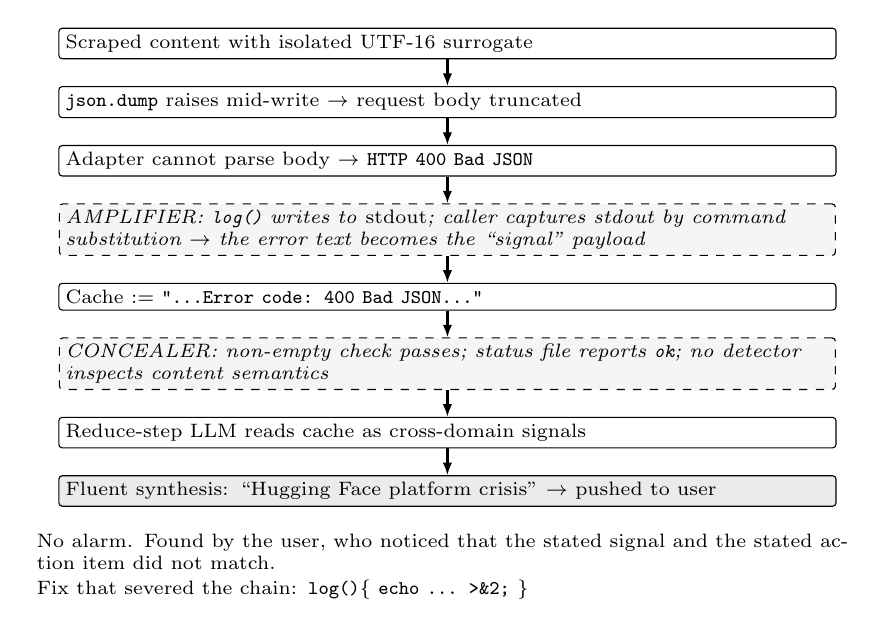
\begin{tikzpicture}[
  node distance=3.4mm,
  box/.style={draw, rounded corners=1.2pt, align=left, inner sep=2.4pt,
              text width=0.80\columnwidth, font=\scriptsize},
  side/.style={draw, dashed, rounded corners=1.2pt, align=left,
               inner sep=2.2pt, font=\scriptsize\itshape,
               text width=0.80\columnwidth},
  arr/.style={-{Latex[length=1.6mm]}, thick}
]
\node[box] (src) {Scraped content with isolated UTF-16 surrogate};
\node[box, below=of src] (trunc)
  {\texttt{json.dump} raises mid-write $\rightarrow$ request body truncated};
\node[box, below=of trunc] (http)
  {Adapter cannot parse body $\rightarrow$ \texttt{HTTP 400 Bad JSON}};
\node[side, below=of http, fill=black!4] (amp)
  {AMPLIFIER: \texttt{log()} writes to \emph{stdout}; caller captures stdout
   by command substitution $\rightarrow$ the error text becomes the
   ``signal'' payload};
\node[box, below=of amp] (cache)
  {Cache := \texttt{"...Error code: 400 Bad JSON..."}};
\node[side, below=of cache, fill=black!4] (conc)
  {CONCEALER: non-empty check passes; status file reports \texttt{ok}; no
   detector inspects content semantics};
\node[box, below=of conc] (llm)
  {Reduce-step LLM reads cache as cross-domain signals};
\node[box, below=of llm, fill=black!8] (out)
  {Fluent synthesis: ``Hugging Face platform crisis'' $\rightarrow$ pushed
   to user};
\node[below=2.2mm of out, font=\scriptsize, text width=0.86\columnwidth,
      align=left] (found)
  {No alarm. Found by the user, who noticed that the stated signal and the
   stated action item did not match.\\[1.2pt]
   Fix that severed the chain: \texttt{log()\{ echo ... >\&2; \}}};

\draw[arr] (src) -- (trunc);
\draw[arr] (trunc) -- (http);
\draw[arr] (http) -- (amp);
\draw[arr] (amp) -- (cache);
\draw[arr] (cache) -- (conc);
\draw[arr] (conc) -- (llm);
\draw[arr] (llm) -- (out);
\end{tikzpicture}
\caption{The D1 pollution chain: one malformed byte becomes a fabricated
industry analysis. Every component behaves as designed. Dashed boxes mark
the amplifier and the concealer (Sec.~\ref{sec:structure}).}
\label{fig:d1}
\end{figure}

\emph{D2: the fabricated remediation.} A watchdog alert was persisted into
chat session history as an ordinary assistant message. Thirty-six minutes
later the user asked an unrelated architecture question. The model attended
across the contaminated context, claimed it had received a system alert
follow-up task, and instructed the user to grant Full Disk Access to a cron
binary. The instruction was ungrounded. Alert traffic and conversation are
different speech acts, and sharing one context window invites the model to
merge them.

\emph{D3: the fabricated success.} A weekly review job whose LLM call failed
fell back to a mechanical line filter. That filter emitted leftover
container headings as review content, and the job recorded that an LLM had
produced the output. The artifact looked plausible for weeks.

\emph{D4: the fabricated release.} An evening digest received the day's
high-alignment papers as enrichment context, without provenance labels. It
inferred that the project must have shipped a release, and announced a
version number that exists only in an internal changelog. True but
unlabelled context produced a false attribution.

The common structure is a \textbf{pollution chain}. A Class A, B, or C
failure deposits non-signal content where a downstream model expects signal.
The model completes fluently. The output has the form of health and the
content of failure.

We define fabrication by absence of grounding, not by inaccuracy. A
fabricated claim can be coincidentally true and is still fabricated.

\subsection{Class E --- Operational omission and forensic blind spot}

The code is correct. An operational step never happened, or the diagnostic
instrument is itself compromised. This is the largest class and holds the
longest silences.

\emph{Omission.} A new daily job was implemented, tested, registered, and
deployed. It never ran, because the final step --- writing the crontab line
--- was a human memory item. Three small defects hid it: the preflight check
grepped for only one of two warning strings; the crontab helper ignored its
install exit code and compared counts with \texttt{<} rather than equality,
reporting success on a rejected install; and a job that never runs produces
no log.

\emph{Self-silencing.} The AI assistant, finishing an alert task, wrote
completion notes into a file named \texttt{HEARTBEAT.md}. To the assistant
this was a scratch filename. To the runtime it was a reserved control file
whose non-empty content activates a heartbeat protocol. Under that protocol
the model replies with a bare acknowledgment token, which the gateway strips
from outbound messages. For 13 hours every user message received an
acknowledgment token that was stripped to nothing. The user received
silence. Every component worked as designed.

\emph{Forensic blind spot.} The longest silence in the corpus, 60 days, was
an external-SSD backup failing with EPERM. Six successive hypotheses were
each falsified by data over several weeks. The breakthrough came from the
operating system audit log, which revealed macOS TCC sandbox denials:
cron-derived processes lacked Full Disk Access.

The methodological finding matters more than the cause. During those weeks
the forensic collectors themselves were being denied and were returning
empty output, which the pipeline recorded as ``normal''. An instrument that
cannot distinguish ``nothing is there'' from ``I was not allowed to look''
manufactures false reassurance. The collectors now capture standard error
separately and tag denied results.

% =====================================================================
\section{Findings (RQ2)}
\label{sec:findings}
% =====================================================================

\subsection{Discovery channel}

Table~\ref{tab:discovery} gives the discovery channel for all 22 incidents.

\begin{table}[t]
\caption{Discovery channel, $n = 22$.}
\label{tab:discovery}
\centering
\footnotesize
\begin{tabular}{@{}l r r@{}}
\toprule
Channel & Count & Share \\
\midrule
Human user-view observation & 13 & 59\% \\
Log forensics (after suspicion) & 4 & 18\% \\
Automated check (preflight or audit) & 3 & 14\% \\
Self-observation (governance auditing itself) & 2 & 9\% \\
\bottomrule
\end{tabular}
\end{table}

The largest single channel is a human reading the product as a user would.
That reading was institutionalized during the study as a weekly 30-minute
review with no coding, covering alert noise, push latency, information
density, and response quality. Typical findings sound like ``this digest
looks shallow'', ``why did I get two windows'', and ``yesterday's analysis
never arrived''.

Automated checks discovered 3 of 22. We report that number rather than an
approximation, and we note that it is partly a selection effect: the corpus
admits only incidents that survived a silent phase with green indicators, so
it excludes everything the checks caught immediately.

The magnitude of the first row is not a selection effect. The system ran
4{,}286 tests, 827 governance checks, and a 19-point preflight, all green
through most of these incidents.

For QA practice, we draw one recommendation. User-view observation is an
observability signal and should receive scheduled time. For QA research, the
open problem is mechanizing part of what that human eye does.
Section~\ref{sec:bench} is our first attempt at measuring progress on that
problem.

\subsection{Silence latency}

Silence spans in the corpus range from 36 minutes to 60 days. The
distribution is not driven by code complexity. Code-level defects were
caught quickly, by tests or by the next scheduled run. The incidents that
survived for weeks lived where no test ran: deployment topology, operating
system policy, the monitoring of monitoring, and gaps between declared and
actual state.

We suggest reading latency as a measure of observational distance. For
silent failures, time to detect dominates time to repair by one to two
orders of magnitude, which makes detection latency a more useful reliability
metric than repair time for this class.

\subsection{Structure of the incidents}
\label{sec:structure}

Nearly every postmortem decomposed into three layers: a \textbf{trigger}
(the external spark, such as a surrogate byte or a transient permission
error), an \textbf{amplifier} (the flaw that spreads it, such as diagnostics
on standard output being captured by command substitution), and a
\textbf{concealer} (the absence that hides it, such as a status file
reporting success or a fail-open guard).

The decomposition has a practical consequence. A fix that addresses only the
trigger is cosmetic. Triggers are unbounded. Amplifiers and concealers are
finite and belong to the architecture. In this corpus the highest-leverage
single fixes were at the amplifier level (one output redirection; one shared
helper replacing twenty copies of an idiom) and the concealer level (failing
loudly with the cause; tagging denied forensic output).

\subsection{What the audit framework prevented}
\label{sec:selfaudit}

Mid-study we audited the governance framework against the first 15
incidents, asking for each whether the framework as it existed \emph{before}
the incident could have caught it, and whether the guards added \emph{after}
block the mechanism from recurring.

\begin{table}[t]
\caption{Self-audit of the governance framework, $n = 15$.}
\label{tab:selfaudit}
\centering
\footnotesize
\begin{tabular}{@{}l r@{}}
\toprule
Question & Result \\
\midrule
Prevented the incident in advance & 0 / 15 \\
Gave partial early warning & 2 / 15 \\
Blocks the mechanism from recurring & 13 / 15 \\
Miss rooted in a dimension never considered & 12 / 15 \\
\bottomrule
\end{tabular}
\end{table}

These are counts over 15 incidents in one system. They are not estimates of
how audit frameworks perform in general.

Within those limits, the pattern is informative. The framework prevented
none of the novel incidents and blocks most of them from recurring. That is
the behavior of a regression suite. Twelve of the fifteen misses were in
categories no invariant had contemplated, which no amount of diligence
within the existing set would have covered. If this generalizes at all, the
implication for QA is that prevention of novel failure classes must come
from somewhere other than the regression apparatus.

% =====================================================================
\section{From Corpus to Benchmark (RQ3)}
\label{sec:bench}
% =====================================================================

Section~\ref{sec:findings} identifies the open problem: the most effective
detector in this study was a human, and mechanizing part of that role
requires a way to measure detectors. We release the corpus as a benchmark
for that purpose.

\subsection{Benchmark construction}

The benchmark consumes the label file described in
Sec.~\ref{sec:labelling}. Each case supplies the artifact text a detector
would see, the expected verdict, and the signal that should fire. Cases are
partitioned into three sets.

\begin{itemize}
  \item \textbf{Category A --- regression (6 cases).} Known \failplausible{}
        patterns drawn from incidents in Table~\ref{tab:corpus}. A detector
        is expected to flag these.
  \item \textbf{Clean controls (4 cases).} Healthy outputs from the same
        jobs. A detector is expected not to flag these, because noise is
        itself a failure of a monitoring tool.
  \item \textbf{Category B --- held out (4 cases).} Real incidents for which
        no detection rule was written. These measure whether a detector
        generalizes beyond the patterns it was built for.
\end{itemize}

Held-out cases are never a pass/fail gate. They are reported.

\subsection{Reference detector and results}

The reference detector is a deterministic pre-filter of five rules over
output text.

\begin{enumerate}
  \item \textbf{Pollution signature.} Error codes or status phrases appear
        in content where topic signal belongs.
  \item \textbf{Credibility mismatch.} A low-tier source is wrapped in
        high-confidence language.
  \item \textbf{Fabrication phrase.} A literal phrase recorded from a real
        fabrication incident appears.
  \item \textbf{Provenance gap.} An equivalence claim is asserted without a
        provenance label.
  \item \textbf{Structural incoherence.} Headings appear without bodies, or
        fields collapse into separators.
\end{enumerate}

\begin{table}[t]
\caption{Reference detector on the benchmark.}
\label{tab:detector}
\centering
\footnotesize
\begin{tabular}{@{}l c l@{}}
\toprule
Metric & Result & Interpretation \\
\midrule
Detection, Category A & 6 / 6 & Known patterns caught reliably \\
False positives, clean & 0 / 4 & No noise on healthy output \\
Misses, Category B & 4 / 4 & No generalization to unseen \\
\bottomrule
\end{tabular}
\end{table}

Every rule is validated by sabotage: the suite disables one rule at a time
and requires the corresponding case to fail. A rule that cannot be made to
fail is vacuous, and we found vacuous checks in this system before
(Sec.~\ref{sec:classc}), so we treat this as mandatory.

The third row of Table~\ref{tab:detector} is the useful result. A
deterministic detector built from known incidents catches known incidents
and generalizes to none of the held-out ones. This is what a regression
engine does, and it mirrors the framework-level measurement in
Sec.~\ref{sec:selfaudit}. Detecting novel \failplausible{} output requires
something other than pattern matching, such as semantic grounding checks or
human review.

We state a limitation about the detector's own nature. A model that judges
another model's output is itself a component of the system, and it inherits
every class in Sec.~\ref{sec:taxonomy}. Our own monitoring component shipped
with a Class B path defect and a sampling artifact that made it report a
truncation that had not occurred. An LLM judge needs the same governance and
sabotage validation as the system it judges.

\subsection{Using and extending the benchmark}

The benchmark runs offline with no model access and no external
dependencies, which makes it usable in continuous integration. The exit code
is a gate: it is zero only if Category A detection is complete, false
positives are zero, and every rule is load-bearing.

We include a contribution protocol. A team adding a case from their own
system supplies the artifact text, the mechanism class, the expected signal,
and a pointer to their postmortem. New \failplausible{} patterns that no
rule targets are added as Category B, where they are reported rather than
silently absorbed into the regression set.

The reason to release this is directly connected to our main limitation. A
corpus from one system cannot establish how often these mechanisms occur
elsewhere. A benchmark that other teams can run and extend can.

% =====================================================================
\section{Threats to Validity}
\label{sec:threats}
% =====================================================================

We organize threats using the four case-study
categories~\cite{runeson2009case}.

\textbf{Construct validity.} \emph{Silent failure} requires a silence span
with concurrently green indicators, and we applied that definition at
postmortem time, which risks hindsight framing. Borderline cases that
produced a loud but causeless alert were included only when the actionable
signal was absent; two or three incidents could reasonably be classified
differently. \failplausible{} is defined by absence of grounding rather than
by inaccuracy. Each construct is operationalized against repository
artifacts: a silence span is a timestamp gap against green audit records,
and a fabricated claim is one with no source in the input context.
Classification is therefore checkable by a third party.

\textbf{Internal validity.} The principal threat is confirmation bias in
mechanism assignment. Both coders were the system's operators, and both
contributed to this paper, so inter-annotator agreement cannot be measured
and no $\kappa$ is reported. This is the study's most significant
limitation. Three factors partially mitigate it. Classes are load-bearing,
so an incorrect class produces a wrong scanner result rather than only a
wrong label. Causal claims were triangulated across at least two sources
before recording. Sabotage validation independently confirms many amplifiers
and concealers by reintroducing the mechanism. Two early incidents were
reconstructed retroactively and are flagged as such in the corpus.

We note one discrepancy for the record. An earlier report of this study
stated that approximately 70\% of incidents were discovered by user-view
observation. The labelled corpus released with this paper gives 13 of 22, or
59\%. The corpus labelling is the later and more careful pass, and it is the
number we use.

\textbf{External validity.} One system, one host operating system, one
operator pair, eight weeks, about 40 jobs. We claim analytical
generalization of the mechanism classes and of the
trigger--amplifier--concealer structure, and we disclaim generalization of
the frequencies. The settings that most bound our results are systems
without a synthesis-and-push pipeline, where Class D frequencies will not
transfer, and teams without an unusually attentive single operator, where
the user-view share will be lower.

\textbf{Reliability.} Every postmortem is a standalone public document. All
counts, dates, and audit results are mechanically derivable from the public
repository at the cited commit window. The AI assistant that helped write
the postmortems also helped write this paper, which raises a narrative-bias
risk. We treat that risk as first class: the human is sole author and final
arbiter, all numbers are repository-derivable, and the findings are
unflattering to the narrator. The framework prevented nothing in advance,
the best detector was a person rather than the automation, and the component
built to close one gap opened another.

% =====================================================================
\section{Conclusion}
% =====================================================================

Eight weeks of complete postmortems from a production LLM agent runtime
yield a five-class taxonomy of silent failures. One class, chained
hallucination, is specific to systems that produce language. In this corpus
a human reading the product found 13 of 22 incidents and automated checks
found 3, while the framework prevented none of them in advance and now
blocks 13 of 15 from recurring.

We release the labelled corpus and a runnable benchmark so that these
numbers can be tested rather than believed. The reference detector's result
on held-out cases is the honest summary of where \failplausible{} detection
stands: reliable on patterns it was built for, and blind to the rest.

% =====================================================================
\section*{Generative-AI Use Disclosure}
% =====================================================================

This research used Anthropic's Claude, accessed through a coding-agent
interface, as an engineering and writing collaborator. It assisted in
triaging and reconstructing incident postmortems, extracting and tabulating
data from the public repository, drafting and editing prose, and proposing
structure. It was not used to generate empirical results, invent data, or
make research claims. Every quantitative figure is mechanically derivable
from the public repository and was verified by the author. The author
defined the research questions, performed the classification, drew the
conclusions, and takes full responsibility for the content, including any
errors. No generative-AI system is an author.

The runtime under study is itself an LLM agent system, powered by separate
Qwen3-class models. The AI collaborator described here is the author's
development tool and not the system studied.

% =====================================================================
\section*{Artifact Availability}
% =====================================================================

The 22 incident postmortems, the labelled corpus
(\texttt{docs/llm\_observer\_ground\_truth.yaml}), the benchmark and its
reference detector, the governance ontology, and the full test suite are
public at \url{https://github.com/bisdom-cell/openclaw-model-bridge}. The
governance engine is separately available on PyPI as
\texttt{openclaw-ontology-engine}. A data inventory maps every number in
this paper to its source in the repository. A preprint of an earlier version
is available as arXiv:2606.14589, disclosed per IEEE preprint policy.

% =====================================================================
\begin{thebibliography}{99}
\footnotesize

\bibitem{huang2017gray}
P.~Huang, C.~Guo, L.~Zhou, J.~R. Lorch, Y.~Dang, M.~Chintalapati, and R.~Yao,
``Gray failure: The Achilles' heel of cloud-scale systems,'' in \emph{HotOS},
2017.

\bibitem{gunawi2018failslow}
H.~S. Gunawi \emph{et al.}, ``Fail-slow at scale: Evidence of hardware
performance faults in large production systems,'' in \emph{USENIX FAST},
2018; extended in \emph{ACM Trans. Storage}, vol.~14, no.~3, 2018.

\bibitem{cemri2025mast}
M.~Cemri, M.~Z. Pan, S.~Yang \emph{et al.}, ``Why do multi-agent LLM systems
fail?'' arXiv:2503.13657, 2025 (preprint).

\bibitem{ranganathan2025inference}
B.~Ranganathan, M.~Zhang, and K.~Wu, ``Enhancing reliability in AI inference
services: An empirical study on real production incidents,''
arXiv:2511.07424, 2025 (preprint).

\bibitem{zhou2025shielda}
J.~Zhou, J.~Chen, Q.~Lu, D.~Zhao, and L.~Zhu, ``SHIELDA: Structured handling
of exceptions in LLM-driven agentic workflows,'' arXiv:2508.07935, 2025
(preprint).

\bibitem{xiao2026air}
Z.~Xiao, J.~Sun, and J.~Chen, ``AIR: Improving agent safety through incident
response,'' arXiv:2602.11749, 2026 (preprint).

\bibitem{taraghi2026mcp}
M.~Taraghi, M.~M. Morovati, and F.~Khomh, ``Real faults in Model Context
Protocol (MCP) software: A comprehensive taxonomy,'' arXiv:2603.05637, 2026
(preprint).

\bibitem{beyer2016sre}
B.~Beyer, C.~Jones, J.~Petoff, and N.~R. Murphy, Eds., \emph{Site Reliability
Engineering}. O'Reilly, 2016.

\bibitem{ezell2025incident}
C.~Ezell, X.~Roberts-Gaal, and A.~Chan, ``Incident analysis for AI agents,''
in \emph{AIES}, 2025; arXiv:2508.14231 (preprint).

\bibitem{owotogbe2026mcpfaults}
J.~Owotogbe, I.~Kumara, W.-J. van~den Heuvel, D.~A. Tamburri, A.~K.
Iannillo, and R.~Natella, ``A taxonomy of runtime faults in Model Context
Protocol servers,'' arXiv:2606.05339, 2026 (preprint).

\bibitem{huang2023hallucination}
L.~Huang, W.~Yu, W.~Ma \emph{et al.}, ``A survey on hallucination in large
language models,'' arXiv:2311.05232, 2023 (rev. 2024).

\bibitem{basiri2016chaos}
A.~Basiri, N.~Behnam, R.~de~Rooij \emph{et al.}, ``Chaos engineering,''
\emph{IEEE Software}, vol.~33, no.~3, pp.~35--41, 2016.

\bibitem{ghosh2022incidents}
S.~Ghosh, M.~Shetty, C.~Bansal, and S.~Nath, ``How to fight production
incidents? An empirical study on a large-scale cloud service,'' in \emph{ACM
SoCC}, 2022.

\bibitem{zheng2023judge}
L.~Zheng, W.-L. Chiang, Y.~Sheng \emph{et al.}, ``Judging LLM-as-a-judge with
MT-Bench and Chatbot Arena,'' in \emph{NeurIPS}, 2023.

\bibitem{runeson2009case}
P.~Runeson and M.~H\"{o}st, ``Guidelines for conducting and reporting case
study research in software engineering,'' \emph{Empirical Software
Engineering}, vol.~14, no.~2, pp.~131--164, 2009.

\end{thebibliography}

\end{document}
